\section{Mass distribution}
\label{sec:mass-distribution}
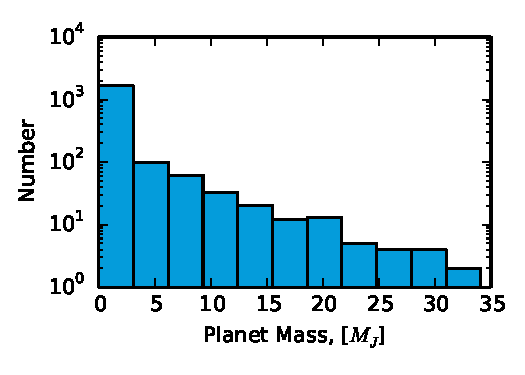
\includegraphics{figures/masshist.pdf}
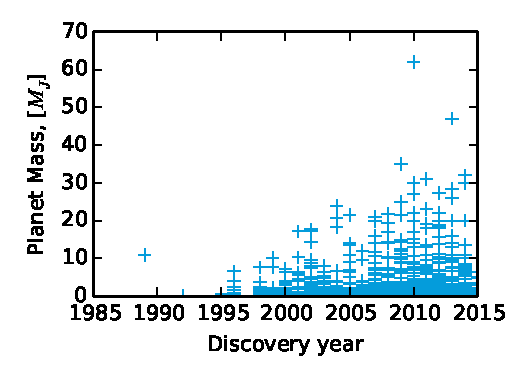
\includegraphics{figures/massyear.pdf}
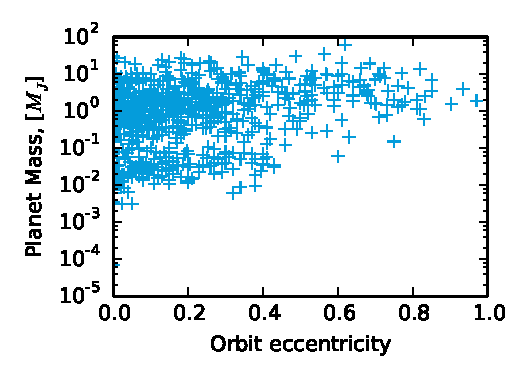
\includegraphics{figures/eccmass.pdf}
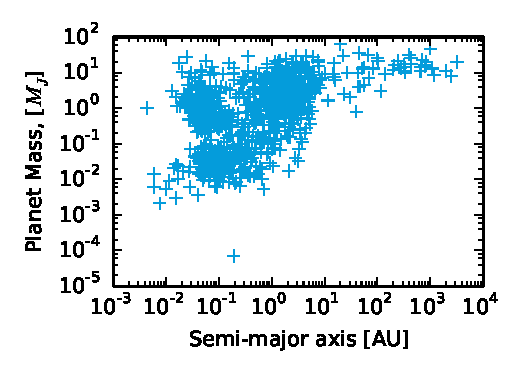
\includegraphics{figures/semimass.pdf}

\section{Semi-major axes}
\label{sec:semi-major-axes}

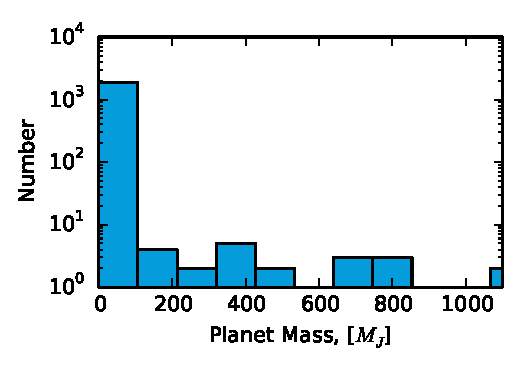
\includegraphics{figures/axishist.pdf}
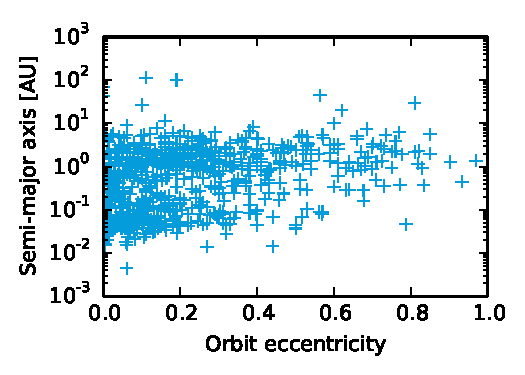
\includegraphics{figures/eccsemi.pdf}

% \section{Atmospheres}
% \label{sec:atmospheres}

% HD\,209458\,b was the first planet to have a spectroscopic signature
% of sodium discovered in its atmosphere, but at an intensity lower than
% was expected, suggesting that high clouds obscure the lower layers of
% the atmosphere. The planet's spectrum is extracted by subtracting the
% stellar spectrum from the overall spectrum.

%%% Local Variables: 
%%% mode: latex
%%% TeX-master: "../project"
%%% End: 
